\chapter{Demonstration Device Overview}\label{ch:overview}

\section{Double-Acting Pneumatic Actuator}
\begin{figure}[h!]
    \centering
    \begin{subfigure}[b]{0.3\textwidth}
        \centering
        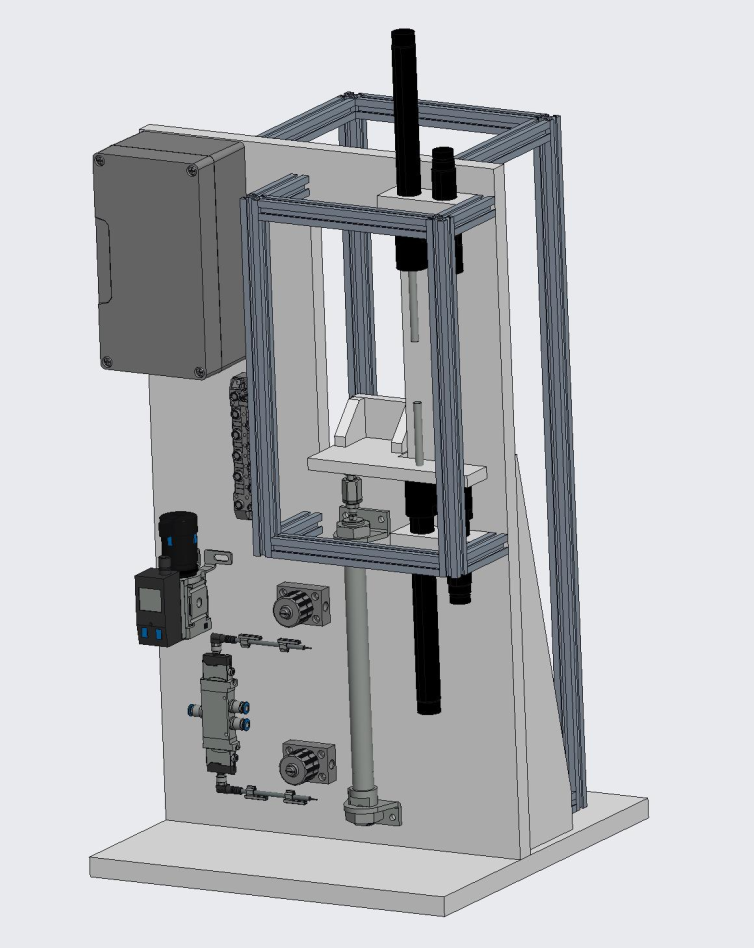
\includegraphics[width=1\textwidth]{model3d.png}
        \caption{3D render of the demonstration device}
        \label{fig:3d}
    \end{subfigure} 
    \hfill
    \begin{subfigure}[b]{0.6\textwidth}
        \centering
        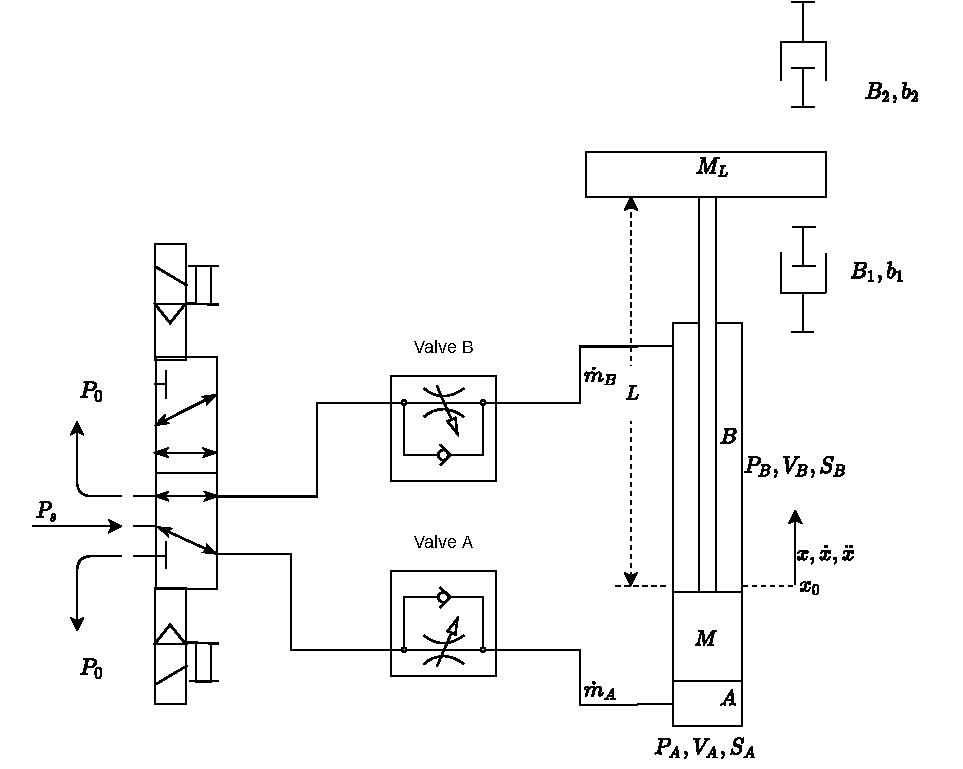
\includegraphics[width=1\textwidth]{system_scheme.pdf}
        \caption{Schematically representation of the demonstration device}
        \label{fig:device_scheme}
    \end{subfigure}
    \caption{Demonstration device}
    \label{fig:device}
\end{figure}

The case study of this thesis is the double-acting pneumatic piston, with a
pneumatic circuit and mechanical assembly driven by a piston.  Figure
\ref{fig:device_scheme} is a schematical representation of the system.
Figure \ref{fig:3d} is a 3D render of the system.

Pneumatic systems use air to transmit power between components in the
circuit. The air is a compressible gas, and we have to consider this when
designing a model. Pneumatic actuators are highly efficient and fast
drives. Using compressed air pneumatic actuator can move with high
velocities and supply nominal force in the kN range. One of the advantages
of a pneumatic system with a piston is that only one supply line is
necessary, giving many opportunities to design and maintain the system.
The basic pneumatic system includes an air reservoir with supplied air,
pressure lines connection, pneumatic actuator and control valve to connect
the supply pressure and actuator. Resistance to movement places a mass that
acts on the piston. 

In this thesis, a double-acting pneumatic actuator, as shown in figure
\ref{fig:device_scheme} was used. Throttling valves A and B regulate the air mass flow to
the piston's chambers. Proportion valve connects supply and ambient
pressure lines to achieve piston control. There are two pairs of dampers
installed to prevent possible destruction impact and simulate different
material penetration resistance.

The demonstration device can be used in stamping, drilling, moving
applications. All system parameters concerning datasheets and measurements
are described in attachment \textit{models/params.m}.

\section{Sensors}

There are eight types of sensors located on the system. Table
\ref{tab:sensors_tab} describes a sensor purpose, signal name in the
datastore, and the signal unit. 

\begin{table}[h!]
    \centering
    \begin{tabular}{|c|c|c|c|}
\hline
\textbf{Sensor} & \textbf{Unit} & \textbf{Description} & \textbf{Name} \\
\hline
Encoder       & m     & displacement                           & LeverPosition \\
Encoder       & m/s   & velocity                               & LeverVelocity \\
Accelerometer & g     & accelerometer on moving part           & AccelerometerMovin\_axisZ/Y \\ 
Accelerometer & g     & accelerometer on static part           & AccelerometerStatic\_axisZ/Y \\ 
Flow Sensor   & l/min & air flow extrusion to A chamber        & FlowExtrusion \\
Flow Sensor   & l/min & air flow contraction from A chamber    & FlowContraction \\
Pressure      & bar   & pressure measurement in reservoir      & AirPressure \\
Microphone    & V     & microphone on upper bumper             & MIC\_uBumper \\ 
Microphone    & V     & microphone on bottom bumper            & MIC\_bBumper \\ 
Microphone    & V     & ambient microphone                     & MIC\_Ambient \\
Temperature   & $^o$C & cylinder temperature measurement       & TempCylinder \\
Temperature   & $^o$C & ambient temperature measurement        & TempAmbient \\
Strain Gauge  & Pa    & strain measurements                    & StrainGauge \\
Proximity     & -     & upper bound detection                  & ProximitySensor\_upper \\
Proximity     & -     & bottom bound detection                 & ProximitySensor\_bottom \\
\hline
    \end{tabular}
    \caption{Sensors overview}
    \label{tab:sensors_tab}
\end{table}

The dataset measured on the system contains almost five thousand
measurements in different operating conditions. Each measurement includes a
10-second recording of moving the pistol up and down. This data was given
in the format of massive files with the ".mat" extension, which was divided
into files contains only one measurement.  The divided dataset is easier to
maintain, and Matlab recommends this type of datastores called Data
Ensemble \cite{data_ensemble}.

The measured examples are shown in figures
\ref{fig:over_examp_1}, \ref{fig:over_examp_3}, \ref{fig:over_examp_3},
and \ref{fig:over_examp_4} .

\begin{figure}[!htb]
    \centering
    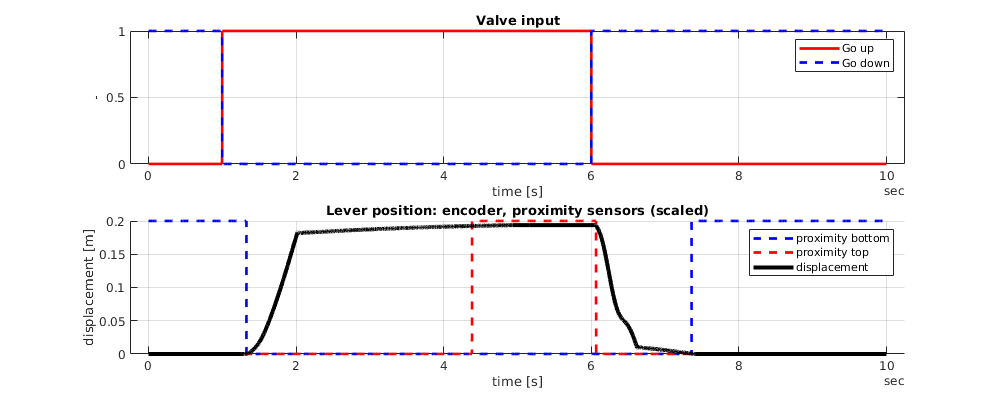
\includegraphics[width=1\textwidth]{overview_data_example_4.png}
    \caption{Example of measured signal}
    \label{fig:over_examp_1}
\end{figure}


\newpage
\begin{figure}[!htb]
    \centering
    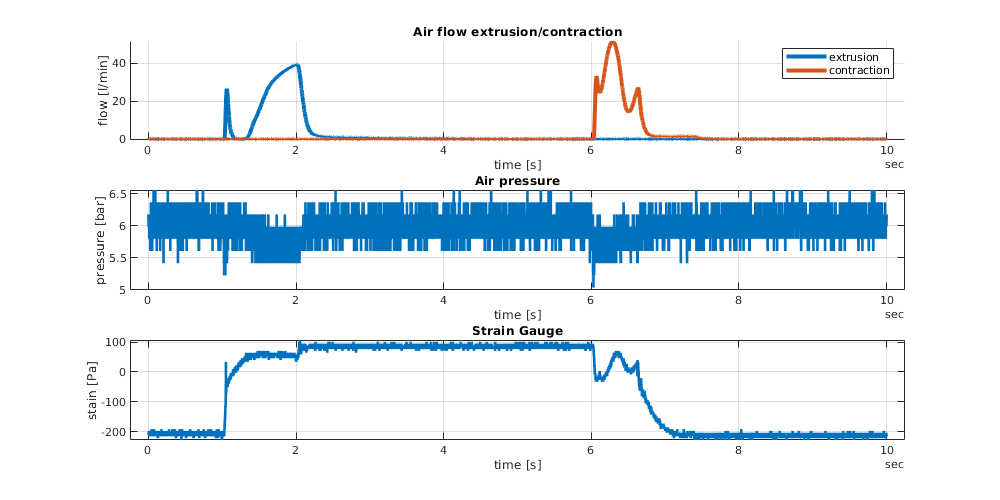
\includegraphics[width=1\textwidth]{overview_data_example_1.png}
    \caption{Example of measured signal}
    \label{fig:over_examp_2}
\end{figure}

\begin{figure}[!htb]
    \centering
    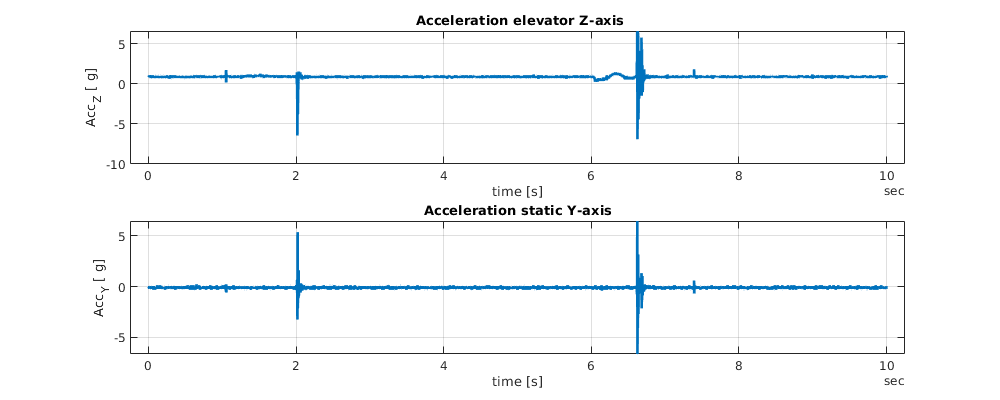
\includegraphics[width=1\textwidth]{overview_data_example_2.png}
    \caption{Example of measured signal}
    \label{fig:over_examp_3}
\end{figure}

\begin{figure}[!htb]
    \centering
    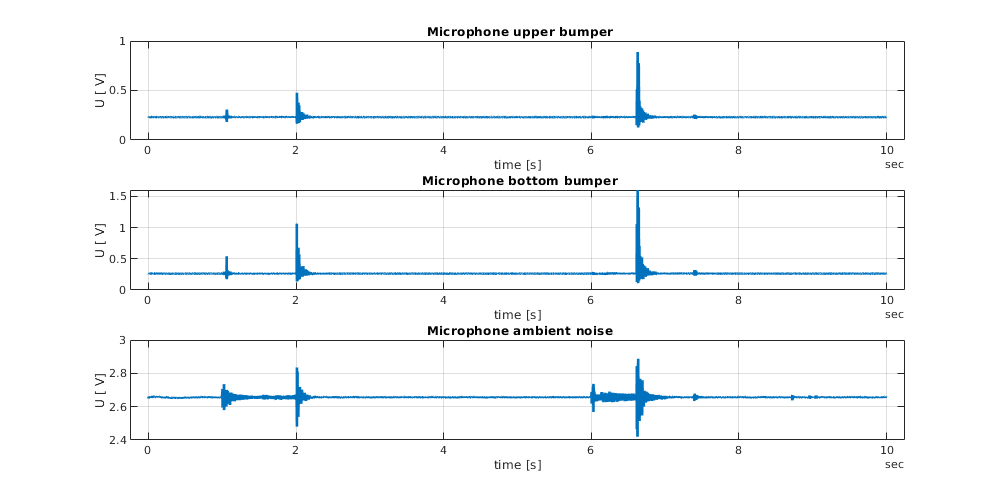
\includegraphics[width=1\textwidth]{overview_data_example_3.png}
    \caption{Example of measured signal}
    \label{fig:over_examp_4}
\end{figure}

\section{Fault Conditions}

The demonstration device contains various settings that were used to
change the system's behavior; these settings are presented in Table
\ref{tab:setting}.

\begin{table}[h]
    \centering
    \begin{tabular}{|c|c|}
        \hline
        \textbf{equipment}  & \textbf{values} \\  \hline
        Throttle valve 1    & adjustment in range 1 to 10 [-] \\
        Throttle valve 2    & adjustment in range 1 to 10 [-] \\
        Small damper upper  & adjustment in range 1 to 10 [-] \\
        Small damper bottom & adjustment in range 1 to 10 [-] \\
        Large dampers       & without adjustment, static value \\
        Load mass           & 0, 1.25, 5, 6.25 [kg] \\
        Supply pressure     & 5, 6 [bar]    \\
        \hline
    \end{tabular}
    \caption{Demonstration device settings equipment}
    \label{tab:setting}
\end{table}


Different loads and material resistance is acting on the pneumatic piston
during various work operations. Setting parameters can be set for each
working operation to run in the so-called health condition. In which the
parameters for effective functionality and extension of component life are
optimally set. However, occasionally there is an undesirable change of the
parameter, which can then cause a fault or inefficient functionality. These
situations need to be corrected and the possible cause pointed out.

\newpage
The measured dataset observes almost 250 different condition situations
where setting parameters were changed to simulate the fault behavior of the
system. Each case has a unique fault code for orientation in the dataset.
Nevertheless, for further development, these fault codes were combined
according to where the fault occurs. Thus combined fault codes were added
to the dataset as labels.

These 20 labels were further used for PdM algorithms:

\begin{itemize}
    \item Healthy
    \item Throttle valve 1
    \item Throttle valve 2 
    \item Small damper bottom
    \item Small damper upper
    \item Large dampers 
    \item And combinations of these faults
\end{itemize}


